%It is recommended that you use pdflatex for compilation

\documentclass[12pt,letterpaper]{article}

\usepackage[pdftex]{graphicx}
\usepackage{float}
\usepackage{ulem}
\usepackage[in]{fullpage} % reduces margins if uncommented
%Why does KIPR require use to use 1in paper?
\usepackage{hyperref}

\pagestyle{empty}

\newcommand{\urlfootnote}[1]{\footnote{\url{#1}}}
\newcommand{\code}[1]{\par\texttt{#1}\par}
\newcommand{\authorInfo}[1]{\gdef\authInfo{#1}}

\title{CBCJVM: Applications of the Java Virtual Machine with Robotics}

\author{Braden McDorman \textit{(beta/catron)}\\
Benjamin Woodruff \textit{(pipeep)}\\
Akshay Joshi \textit{(axyjo)}\\
Jonathan Frias \textit{(freakinjonathan)}}

\authorInfo{Norman Advanced Botball \texttt{braden@betabot.org}\\
Fletcher High School \texttt{odetopi.e@gmail.com}\\
American Community School of Abu Dhabi \texttt{me@akshayjoshi.com}\\
Robert E.~Lee High \texttt{freakinjonathan@gmail.com}}
%we should clean up the way the author list is formated

\begin{document}

\makeatletter
\noindent\begin{minipage}[l]{.8\textwidth}\begin{flushleft}\begin{small}
\textbf{\@title}\vspace{.75em}

\@author\vspace{.5em}

\authInfo
\end{small}\end{flushleft}\end{minipage}\vspace{.25in}
\begin{center}
\begin{Large}
\textbf{\@title}
\end{Large}
\par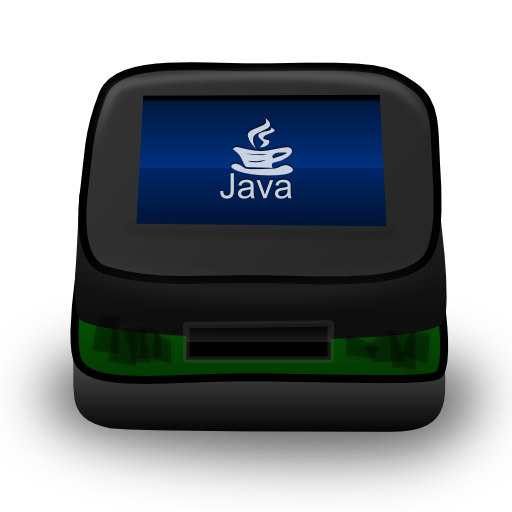
\includegraphics[height=.5in]{CBCJava.png}
\end{center}
\makeatother

\section{Concept and Background}

\subsection{Thesis}

The Botball tournament requires programmers to rapidly develop and prototype programs. However, a disconnect is visible between the language and the tools provided and the goals of the game. Although very fast, C is generally considered to be a low-level language, making it what many of us believe to be the wrong tool for the job. The result is buggy programs, cluttered code, and a lack of flexibility in user libraries. CBCJVM is the product of the realization that although slower, interpreted Object-Oriented programming languages are better for the type of prototyping used in the Botball competition. As KIPR has stated many times, it is highly unlikely that the CBC will ever be officially changed from C \urlfootnote{http://community.botball.org/forum/miscellaneous/suggestions-and-bugs/can-there-be-kiss-c-rather-kiss-c}. CBCJVM shares many of the same goals as Nease's CBCLua, but is aimed at a wider audience. It features monthly releases, detailed documentation, and support for more than just one language. CBCJVM is not just a port of JVM to the CBC. It encompasses a group of libraries and tools to compete with (and at oftentimes, surpass) those offered by KISS-C.



\subsection{License}

CBCJVM is licensed under the GPLv3\urlfootnote{http://gplv3.fsf.org/}. This license requires that you distribute the source code of any modifications of CBCJVM along with any binary version of it that you distribute. We, the authors of CBCJVM, believe this constitutes a fair and just agreement. You are also permitted to use CBCJVM under any future version of the GPL that you wish.



\subsection{Languages}

The CBCJVM originally went under the name ``CBCJava", but as the project grew, it was soon realized that using the JVM only for Java was a waste. The Java Virtual Machine has become a de facto standard of virtual machines, and almost every interpreted language imaginable has some port to the JVM, and these languages typically have support for interfacing with Java libraries. The JVM is fast, taking advantage of Just-In-Time compilation and various other optimizations, making its performance somewhat comparable to C++ and C. However, the performance is  in no way better than a native language. CBCJVM has been used with JavaScript (via Mozilla Rhino) and Scala (which compiles directly to Java byte-code), but it can be used with many other languages such as Ruby, Python, Lua, and even LOLCODE. While it cannot always match the performance of native interpreters for these languages (such as WebKit (JavaScript), CPython, or the standard Lua interpreter), it offers a fast way for teams to get up and running with these high level languages. Furthermore, CBCJVM already includes a set of powerful libraries that can be used in conjunction with these languages to help teams that would otherwise be on their own with a language (not everyone can port and develop libraries in a language entirely by themselves and have it work well... *cough* Nease, CBCLua *cough*).

Due to the limited scope of this document, and the large differences in how various JVM languages manage their bindings to Java code, we will not discuss the specifics of running these languages. Please see the Ending Notes for information on finding help for doing this.



\subsection{Libraries}

Rather than being a straight port of the JVM to the CBC, CBCJVM includes libraries developed on top of the JVM. These libraries allow access to the KISS-C libraries via the Java Native Interface (JNI), allowing you to control motors, read sensors, and so on. Although bugs occasionally show up in this low-level communication layer, we believe that our implementation is complete and stable enough to be used on a day-to-day basis. These low level functions are available in the \texttt{cbccore.low} package.

On top of this, we have classes that make the low level functions more object-oriented, and use camelCase for function names, rather than KISS-C's underscore{\_}naming{\_}system. The majority of CBCJVM's classes use these camelCased classes, and so should you. That said, all simulation happens in this \texttt{cbccore.low} package. Thus, there is no loss in functionality by using the \texttt{cbccore.low} package. There exist two obvious reasons for the use of the \texttt{cbccore.low} package in your own code:
\begin{itemize}
\item Ease of porting from KISS-C code.

\textit{Although the best option would be to port your code to CBCJVM utilizing the new APIs, in an object-oriented fashion, the \textit{cbccore.low} package can be used to do a quick ad-hoc port of code, due to it's similarities to the KISS-C's API.}

\item The use of some feature where no high-level, camelCased class exists to handle it yet.

\textit{We try our best, but as a (currently) small development team, there is the possibility that we have overlooked some functions in our porting efforts. However, the best option would be to fork\urlfootnote{http://help.github.com/forking} our github repository\urlfootnote{http://github.com/catron/CBCJVM}, add that functionality yourself, and submit a pull request\urlfootnote{http://github.com/guides/pull-requests}, or report it in our github issue tracker \urlfootnote{http://github.com/catron/CBCJVM/issues} and wait for a fix.}

More information regarding these libraries can be found in the \textit{Features and Internals} section.
\end{itemize}



\pagebreak
\section{Features and Internals}

\subsection{Running the JVM}

CBCJVM uses a lightweight JVM called JamVM\urlfootnote{http://jamvm.sourceforge.net}. JamVM is designed for embedded platforms, such as the Linux-running Chumby used in the CBC. JamVM gives us excellent compatibility with Sun's Java standard library because it uses GNU Classpath\urlfootnote{http://www.gnu.org/software/classpath} for its standard library. This allows us to run generated byte code on the computer and CBC with no modification. Our simulator exploits this cross compatibility by replacing the \texttt{cbccore.low.*} libraries at runtime.



\subsection{Simulator}

As mentioned, our simulator replaces classes loaded by \texttt{cbccore.Device} at runtime if it detects that it is running on a computer. These simulated Device classes then update a Simulator GUI singleton. This is done automatically and is transparent to the user. The simulator is still in an early state, but its architecture allows room for fast and easy expansion.

\begin{figure}[h]
\begin{flushright}
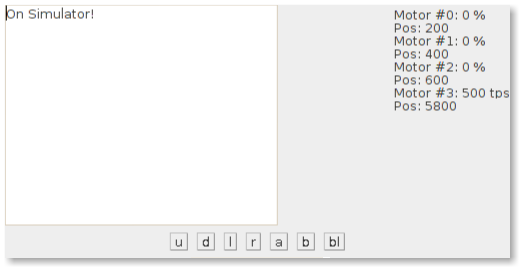
\includegraphics[width=.75\textwidth]{simulator.png}
\end{flushright}
\caption{\textit{The CBCJVM simulator, demonstrating motor simulation. The simulator also has support for framebuffer simulation (not shown).}}
\end{figure}


\subsection{Frame Buffer Access}

One of the more unique features of CBCJVM is the ability to draw to the CBC's $320 \times 240$ screen. This is accomplished by writing RGB16 data to the \textsl{/dev/fb0} pipe provided by Linux. A custom-made library built specifically for CBCJVM gives you helper classes such as pixmaps (Pixel Buffers) with simple drawing functions and Image data types. The frame buffer is also simulated on the computer, allowing you to test your drawing code directly in the simulator. You can find more details about CBCJVM's frame buffer library in \texttt{cbccore.display} package.



\subsection{Movement Library}

Never again will you have to write your own movement library CBCJVM includes an extensible Object-Oriented library. Its plug-in based architecture allows easy adoption for any piece of hardware: motor based or Create based. In addition, a simulator plug-in is currently in development, meaning that you will be able to have a KISS-C style simulation system that can be used with any JVM language. Plug-ins are essentially stubs, telling the DriveTrain class (the center of the movement library) what functions to call for a specific piece of hardware. By making all your movements through this library, you can take advantage of features such as position tracking. The movement library can be found in \texttt{cbccore.movement}.

\subsubsection{Example Code}
\begin{verbatim}import cbccore.movement.DriveTrain;
import cbccore.movement.plugins.create.CreateMovementPlugin;
/* There is also a MotorMovementPlugin located at:
 * cbccore.movement.plugins.motor.MotorMovementPlugin
 * for traditional Lego-chassis robots. You can read more
 * about this in the later mentioned JavaDoc files.
 */

public class MovementLibraryExample {
    public static void main(String[] args) {
        //create a new DriveTrain instance:
        DriveTrain dt = new DriveTrain(
            new CreateMovementPlugin(
                    //Wrap a plugin in the DriveTrain class
                1.0 //Efficiency, a 'fudge' factor
                , true //"Full" mode, as defined by KISS-C
            )
        );
        /* You are free to extend the DriveTrain class as you wish,
         * using any "plug-in" you wish with the extended version.
         */
        
        //move one meter forward, half speed:
        dt.moveCm(100.0, 0.5*dt.getMaxCmps());
        
        //rotate 90 degrees, counter-clock-wise, half speed:
        dt.rotateDegrees(90.0, 0.5*dt.getMaxDegreesPerSec());
        
        System.out.println(dt.getPosition().getAngleDegrees());
        //will print out 90.0
    }
}
\end{verbatim}


\subsection{Configuration System}

``Configurators" can get input from a user for several options using buttons, touch sensors, or even analog sensors using an \texttt{cbcccore.\-sensors.\-analog.\-AnalogBooleanAdapter}. This is accomplished by passing an array of options along with an array of acceptable \texttt{IBooleanSensor}s to use, then mapping each option to a unique sensor. Using Configurators allows a programmer to quickly build menu systems based off of the inputs their robot can handle.



\subsection{Eclipse Integration}

Ease of use being of the utmost importance to our team, CBCJVM's Eclipse\urlfootnote{http://www.eclipse.org/} plug-in allows you to download to your CBC via a network or via a flash drive. Eclipse's built in documentation, code completion, and automatic build system allow for you to develop code even faster. Eclipse also provides thousands of plug-ins for integration with software development processes such as version control with Git and Subversion (svn). When downloading over the network there is no need to recompile your program; just simply press run again.

\begin{figure}[H]
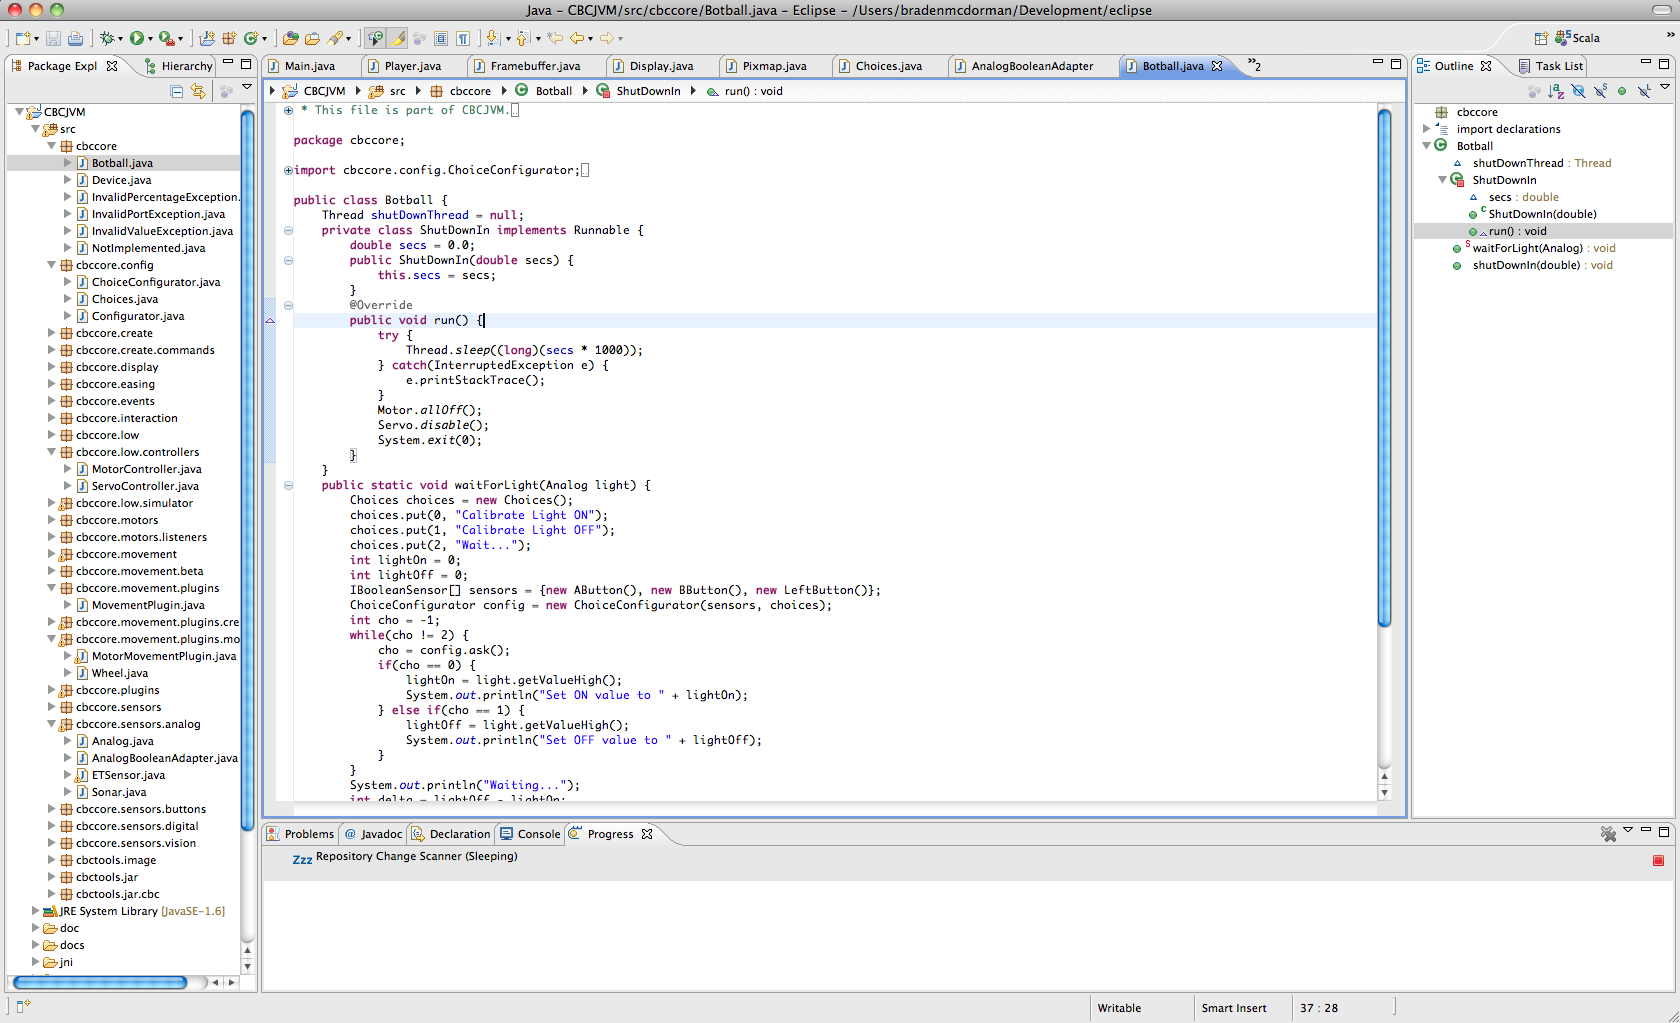
\includegraphics[width=\textwidth]{eclipse.png}
\caption{\textit{CBCJVM being edited in the Eclipse IDE}}
\end{figure}


\subsection{Using CBCJVM Without Eclipse}

There is no requirement to use Eclipse, and it is possible to use the features provided in the Eclipse plug-in without Eclipse.



\subsubsection{Networked Downloads}

A command-line based version the network download tool is available. This tool is built automatically along with the rest of CBCJVM (see setup section for more information). This tool can be found in \texttt{CBCJVM/\-consoleDownload/\-bin/\-Download.\-class}. It can be executed by navigating into the \texttt{CBCJVM/\-consoleDownload/\-bin/} directory with a terminal/command-line, and running the command: \code{java Download <ip-address> <target-directory>} Replacing \texttt{<ip-address>} with the CBC's IP, and \texttt{<target-directory>} with the directory you plan to download. More information on finding the CBC's IP address and networking with the CBC can be found in the 2009 Nease-Norman CBC hacking paper\urlfootnote{http://bit.ly/nn-cbc09}.

\pagebreak
\section{Setup}

\subsection{Background Information}

It is strongly recommended you use CBCJVM on a POSIX compliant operating system such as Linux or Mac OS X. On Windows, everything should work, except for the few Bash-based build scripts (the build process is mainly Ant and Maven based). Complete Windows support is a priority, and should be an easy project for anyone who wishes to take on the task.

\textbf{Warning:} Build instructions may change over time. Therefore, it is always a good idea to consult the CBCJVM wiki\urlfootnote{http://wiki.github.com/catron/CBCJVM/installsetup} for the latest information.

\subsection{Ubuntu Setup}

All of these commands, unless otherwise specified, are to be executed in a Bash (terminal) environment. On a fresh Ubuntu install, that would be found under the top left ``Applications" menu, ``Accessories", ``Terminal". If a command asks for your password, it is referring to your root (administrative) password. If you have no idea what this means, please contact your system administrator.
\begin{enumerate}
\item Open the ``Software Sources" application by going to the ``System" menu at the top left of your screen, ``Administration", ``Software Sources"
\item Ensure that the box ``Community-maintained Open Source software (universe)" is checked. If it is not, check it.
\item Close the window. If you are prompted to update your package list, click the ``Reload" button.
\item Check to see if you have a copy of JDK 6 by running:
      \code{\$ javac -version}
      You should see something like:
      \code{\$ javac 1.6.0{\_}18}
      If it gives a version prior to 1.6.x{\_}x, update your system. If it complains that \texttt{javac} is not found, run
      \code{\$ sudo aptitude install default-jdk}
\item Now, install the additional dependencies:
      \code{\$ sudo aptitude install ant git-core maven2}
      If you already have one of those pieces of software, you can still run the command without fear. Aptitude won't attempt to reinstall the software.
\item Navigate into the directory you want the repository folder to be downloaded to, making a new one if necessary; Eg:
      \code{\$ mkdir "$\mathtt{\sim}$/myFolder"\\
            \$ cd "$\mathtt{\sim}$/myFolder"}
\item Pull (download) a copy of CBCJVM:\par
      \begin{itemize}
          \item Download the latest version (possibly unstable):
                \code{\$ git clone git://github.com/catron/CBCJVM.git \\
                      \$ cd CBCJVM}
          \item Download a specific (``stable") version:
                \code{\$ git clone git://github.com/catron/CBCJVM.git \\
                      \$ cd CBCJVM \\
                      \$ git tag -l \\
                      \$ git checkout 10.6}
                (\texttt{git tag -l} is optional, it will list all available versions. Replace `10.6' with whichever version number you desire.)
      \end{itemize}
      If you are unsure about which version you should download, we recommend that you consult someone on the Botball community chat\urlfootnote{http://community.botball.org/irc}.
\item Compile CBCJVM:
      \code{\$ sh BuildEverything.sh}
\item The CBC installer and corresponding README file can now be found in \texttt{CBCJVM/\-installer/\-install}.
\end{enumerate}



\subsection{Mac OS X Setup}

All of these commands, unless otherwise specified, are to be executed in a Bash (terminal) environment. The default Mac OS X terminal can be found in your ``Applications" folder, ``Utilities", ``Terminal". These steps should work on any version of OS X, but we can only verify them on on Snow Leopard (10.6).
\begin{enumerate}
\item If you haven't already\footnote{If you have the ``Developer" folder in the root directory (\texttt{/}) of your drive (usually labeled ``Macintosh HD"), this probably means that you have already installed the Apple Developer Tools}, download and install the latest version of the Apple Developer Tools (XCode et al.)\urlfootnote{http://developer.apple.com/technologies/xcode.html} available for your system. Although it will work, please note that you do not need the ``iPhone" version. It simply contains more packages that are relevant to iPhone OS development and therefore is larger than the ``Mac" specific version.
\item If you haven't already, download and install MacPorts\urlfootnote{http://www.macports.org/install.php} by following the steps provided on its website.
\item Install required tools for building CBCJVM
      \code{\$ sudo port install apache-ant git-core maven2}
\item Navigate into the directory you want the repository folder to be downloaded to, making a new one if necessary; Eg:
      \code{\$ mkdir "$\mathtt{\sim}$/myFolder"\\
            \$ cd "$\mathtt{\sim}$/myFolder"}
\item Pull (download) a copy of CBCJVM:\par
      \begin{itemize}
          \item Download the latest version (possibly unstable):
                \code{\$ git clone git://github.com/catron/CBCJVM.git \\
                      \$ cd CBCJVM}
          \item Download a specific (``stable") version:
                \code{\$ git clone git://github.com/catron/CBCJVM.git \\
                      \$ cd CBCJVM \\
                      \$ git tag -l \\
                      \$ git checkout 10.6}
                (\texttt{git tag -l} is optional, it will list all available versions. Replace `10.6' with whatever version number you desire.)
      \end{itemize}
      If you are unsure as to what version you should download, it is recommended that you consult someone on the Botball community chat\urlfootnote{http://community.botball.org/irc}.
\item Compile CBCJVM:
      \code{\$ sh BuildEverything.sh}
\item The CBC installer and corresponding README file can now be found in \texttt{CBCJVM/\-installer/\-install}.
\end{enumerate}



\subsection{CBC Setup}

After compiling CBCJVM on your computer or downloading a pre-compiled binary, you must setup CBCJVM on all of the CBCs you wish to use it on.

\textbf{Warning:} This \uline{will only work on a CBCv2}. It \uline{will not} work on a CBCv1, and it \uline{may or may not} run on future versions of the CBC. Future versions of CBCJVM \uline{may or may not} be compatible with different devices. Backwards compatibility \uline{is not guaranteed}. \textbf{CBCJVM comes with no warranty}, and runs the \emph{slim} possibility, as do all CBC mods, of turning your CBC into a very expensive paperweight. \uline{Neither the CBCJVM developers nor KIPR are responsible for you bricking your own device, and it is at KIPR's sole discretion whether or not to fix it}. That said, CBCJVM avoids modifying certain portions of your CBC and attempts to remain as encapsulated as possible, making it improbable that it would damage your device.



\subsubsection{Install}

\begin{enumerate}
\item Copy the contents of the \texttt{CBCJVM/installer/install} directory to the root directory (\texttt{/}) of a flash drive.
\item Load \texttt{CBCJVMInstall.c} in the ``Programs" section of the CBC (cbcui).
\item Run.
\end{enumerate}



\subsubsection{Cleanup}

\begin{enumerate}
\item Delete everything copied to the flash drive.
\end{enumerate}



\pagebreak
\section{Ending Notes}

\subsection{Tomorrow}

Tomorrow! Tomorrow! / I love ya Tomorrow! / You're always / A day / A way!\footnote{Song taken from Annie (the musical). Lyrics were written by Martin Charnin. We believe that the limited use combined with the commentary use of this snippet of lyrics qualifies under ``Fair Use" law.}

\subsubsection{SemiSim}

CBCJVM currently has a simulator, which is especially useful since you can use any JVM debugger of your choice. SemiSim would be a continuation of the Simulator, but all motor and servo commands (from \texttt{cbccore.low}) would be forwarded to a CBC over network. That way, you have the best of both worlds\ldots You can debug your program using a full debugging tool, and execute it on the CBC seamlessly.



\subsubsection{Google Voice Integration}

Google Voice connectivity would allow a CBC to send and receive SMS (text) messages via WiFi, allowing for some interesting design ideas. It would most likely be accomplished with Google Voice Java\urlfootnote{http://code.google.com/p/google-voice-java/}. It could be integrated into CBCJVM directly, allowing a background daemon to handle requests you register with the manager.

Imagine running your robot by simply sending a SMS message to it, or being able to quickly gather information from your CBC while it is still running. This would only be the start. There could be all sorts of unforeseen possibilities for this technology. This does not necessarily have to be done through Google Voice, as it could be done as an IRC or Jabber (a free and open IM protocol). Better yet, it could be done in a pluggable fashion, allowing people to use any web technology of their choice to communicate with it. Imagine a Twittering robot\ldots

\textit{``Picked up the red tribbles! I'm going to head to the basket now!"}

\textit{``The Nease iRobot Create robot is following me @FletcherHighLegoBot, why aren't you?"}



\subsection{Finding Documentation with JavaDoc}

After running the build script, a series of HTML pages will be generated in \texttt{CBCJVM/\-cbc/\-CBCJVM/\-doc}. You can open the file \texttt{index.html} from that directory with your favorite web-browser. This documentation is automatically generated from the CBCJVM source code, and is rebuilt with each execution of the build script.

\begin{figure}[h]
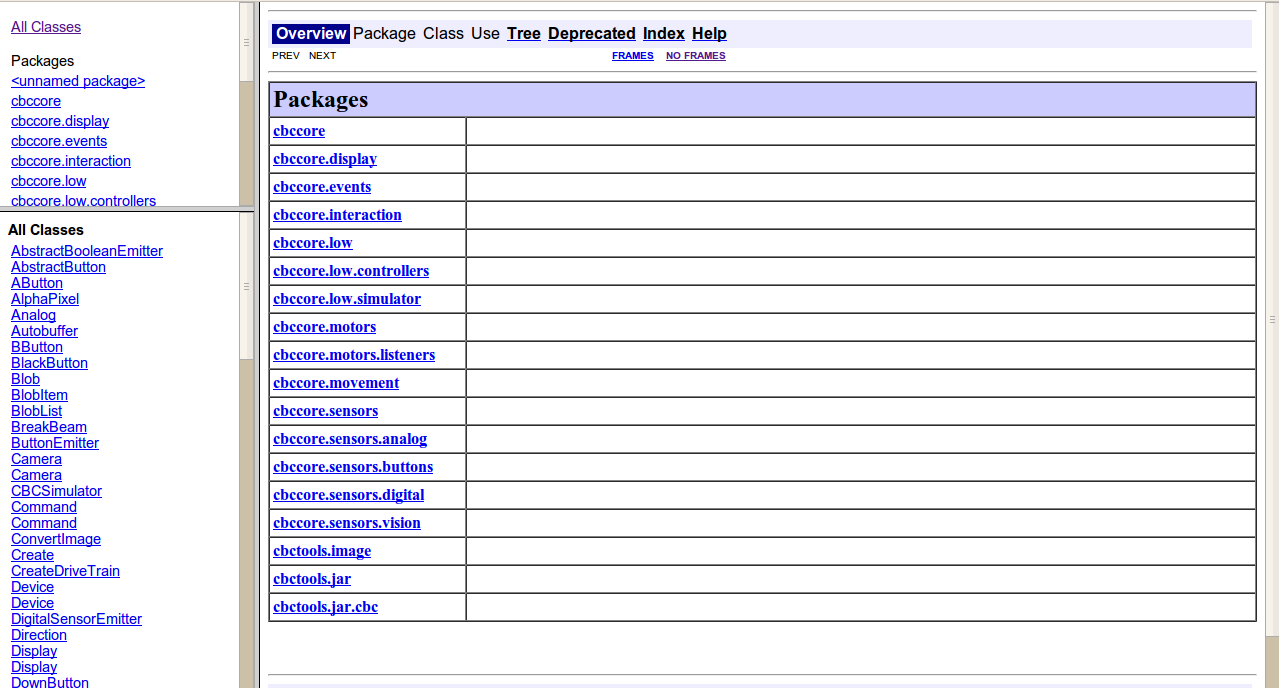
\includegraphics[width=\textwidth]{javadocs.png}
\caption{\textit{The CBCJVM JavaDocs. The top left frame contains CBCJVM specific packages. The bottom left frame contains CBCJVM specific classes. The large frame is used to display information about the currently selected package or class.}}
\end{figure}

For regular users of Java, this should look familiar. This is because official JavaSE/\-ME/\-EE documentation is built using the same tool, JavaDoc. This generated documentation can be found on Sun's website\urlfootnote{http://java.sun.com/javase/6/docs/api}. All of the classes and methods found there should be available on the CBC, with the notable exception of AWT/\-Swing (the packages are actually there, but the CBC lacks a windowing server, making them useless), and a few other minor features not yet available in JamVM/\-GNU-Classpath (such as \texttt{System.\-nanoTime()}).



\subsection{Finding Help on the Internet}

This document cannot cover everything regarding CBCJVM or the technologies surrounding it. It only begins to scratch the surface. The Internet is an incredibly useful tool, but it pays to know where to look. This section attempts to address this, but above all, remember that Google is your friend.



\subsubsection{General Programming and Java Specific Help}

There exist a number of web sites that can help you locate general information on programming, theory and practice. A few of the best resources are listed here:
\begin{itemize}
\item \url{http://en.wikibooks.org/wiki/Java_Programming}\\
      Wikipedia also contains various programming articles, all of great quality. The are numerous Wikipedia articles on Programming Theory.
\item \url{http://www.stackoverflow.com}\\
      A question-and-answer website for all types and kinds of programming. Search before asking a question. Registration \textit{(free)} is required to ask questions.
\end{itemize}



\subsubsection{CBCJVM and Botball Specific Help}

\begin{itemize}
\item \url{http://community.botball.org}\\
      As if this one hasn't been plugged enough. Features a question-and-answer style forum. Registration \textit{(free)} is required to ask questions.
\item \url{irc.mintirc.net} \texttt{{\#}botball} \textbf{or} \url{http://community.botball.org/irc}\\
      Pull up your favorite IRC client and join. Real-time community chat. Due to the limited number of CBCJVM users at the moment, people living in countries other than the US with different timezones may have trouble finding someone they can chat with. Registration \textit{(free)} is not required, although suggested.
\item \url{http://wiki.github.com/catron/CBCJVM}\\
      The official repository for all CBCJVM-specific information.
\item \url{http://github.com/catron/CBCJVM/issues}\\
      If you find a bug in CBCJVM (which admittedly, in its early state, is not hard to do), or have a feature request, this is the place to report it/suggest it. Registration \textit{(free)} is required to report questions.
\end{itemize}

\end{document}